\section{Angewandte Ansätze für die Erkennung von Design Patterns}

Bei der Erkennung von Design Patterns in Quellcode wurden verschiedene Verfahren entwickelt werden, die auf unterschiedlichen Methoden beruhen, um das gesetzte Ziel zu erreichen.
Yarahmadi et al.~führten in ihrer Arbeit eine Untersuchung über die Methoden, die angewandt worden, um Design Patterns in Quellcode zu erkennen, und kategorisierten diese~\cite[S. 5805]{yarahmadi2020design}.

\begin{figure}[h]
    \centering
    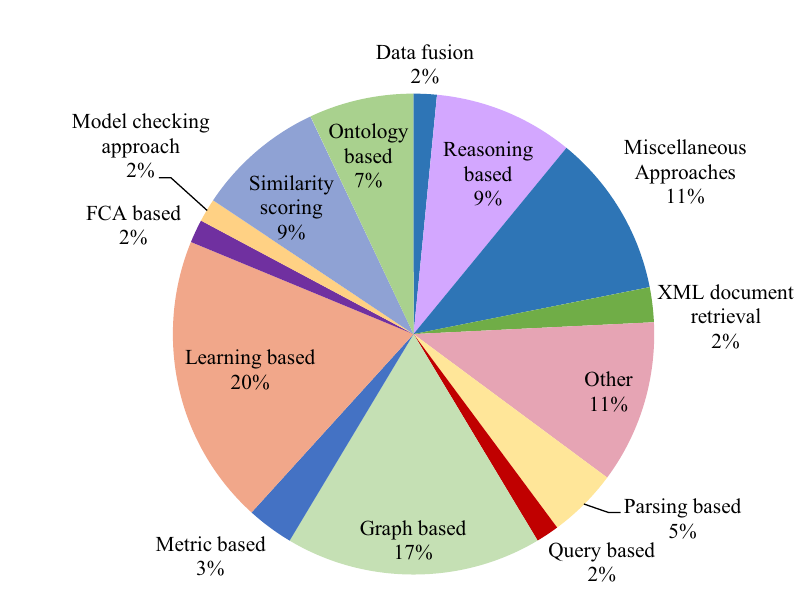
\includegraphics[scale=0.5]{figures/approches_distribution.png}
    \caption{Verteilung der Kategorien der Ansätze für die Erkennung von Design Patterns in Quellcode}
    \label{fig:approach_dist}
\end{figure}

Wie aus Figur~\ref{fig:approach_dist} zu entnehmen ist, lassen sich die entwickelten Prozesse auf eine begrenzte Menge an Kategorien eingestuft werden.
In dieser Sektion der Arbeit werden die vier größten Kategorien aus Figur~\ref{fig:approach_dist} genauer erläutert und es werden exemplarisch Arbeiten diskutiert,
die in die jeweilige Kategorie zugeordnet werden können. 

\subsection{Graphen-basierende Ansätze}

Die Methodik der Reduktion stellt in der Berechenbarkeitstheorie einen Ansatz dar, um Lösungswege für neue unbekannte Probleme zu entwickeln. Dabei wird durch einen Algorithmus das unbekannte Problem in ein bereits gelöstes Problem, dessen Lösungsweg bereits vorhanden ist, umgewandelt.
In Graphen-basierenden Methoden für die Erkennung von Design Pattern in Quellcode wird diese angewendet, um Quellcode in Graphen zu transformieren und diese Graphen werden als Eingabe für diverse Graphenalgortihmen verwendet.

\pagebreak

Formell betrachtet ist ein Graph definiert als~\cite[S. 9]{Siu1998IntroductionTG}:
\begin{align*}
& \text{G} = \{V(G), E(G)\}
&\\
&\text{mit}
&\\
&G : \text{der zu betrachtende Graph}\\
&V (G): \text{Nicht leere Menge von Knoten in G}\\
&E (G): \text{Menge an ungeordneten Tupeln von distinkten Elementen von V (G)}
\end{align*}

Der Quellcode selbst ist als roher Text zu betrachten, welches verschiedene Entitäten wie Klassen, Objekte und Schnittstellen beinhaltet, und definiert, wie diese miteinander interagieren. Als Graph $G$ werden die Entitäten aus dem Quellcode als Knoten $V (G)$ und 
die Relationen und Interaktionen wie Vererbung oder Methodenaufrufe werden als Kanten $E (G)$ dargestellt.
Hierbei stellt Unified Modeling Language (UML) eine in der Software-Entwicklung verbreitete Modellierungssprache dar und definiert verschiedene Arten von Graphen dar, um Software und andere Systeme zu modellieren.
Die Diagramme aus der UML-Domäne werden in diesem Kontext als Graphen aufgefasst, da diese aus einer Menge aus Kanten und Konten bestehen und anhand der obigen Definition als Graphen interpretieret werden können.
Eine Diagrammart aus der Domäne, welches eingesetzt wird, um objektorientierte (OO) Software-Systeme zu modellieren, sind Klassendiagramme.
Klassendiagramme beschreiben, wie Klassen und deren Relation zueinander im Kontext des Paradigmas der OO-Programmierung aufgefasst werden.
Pradhan et al.\ nutzen Klassendiagramme als Eingabe für ihre entworfene Methode und generieren diese für das zu analysierende Software-System und Implementierung von Entwurfsmustern, die als Referenz genutzt werden~\cite[S. 2]{7346680}.
Diese werden als gerichtete Graphen erfasst, wobei die Klassen als Knoten und die Assoziation wie Vererbung zwischen diesen als Kanten darstellen. Zusätzlich werden die Kanten je nach Art der Assoziation unterschiedlich gewichtet~\cite[S. 2]{7346680}.
Im weiteren Verlauf werden mögliche Menge Kandidaten aus dem Graphen des Software-Systems als dessen Subgraphen durch die Eigenschaft der Graphenisomorphie extrahiert und anhand der normalisierten Kreuzrelation der Maß der Übereinstimmung bestimmt~\cite[S. 3]{7346680}.
Graphenisomorphie beschreibt, ob zwei Graphen die strukturell identisch sind, sodass jede Kante des einen Graphen einer Kante im anderen Graphen entspricht und umgekehrt~\cite[S. 10]{Siu1998IntroductionTG}. Die normalisierten Kreuzrelation ist ein Maß, dessen Wertebereich zwischen 0.0 und 1.0 definiert ist.
Je näher der Wert an 1.0, desto identischer sind die zwei Graphen.

%TODO: Add this file:///home/memi/Downloads/Yu,%20Dongjin_%20Zhang,%20Yanyan_%20Ge,%20Jianlin_%20Wu,%20Wei%20-%20[IEEE%202013%20IEEE%2037th%20Annual%20Computer%20Software%20and%20Applications%20Conference%20(COMPSAC)%20-%20Kyoto,%20Japan%20(2013.07.22-2013.07.26)]%20201%20(2013,%20IEEE)%20[10.1109_COMPSAC.2013.92]%20-%20libge.pdf

\subsection{Maschine Learning Ansätze}


\subsection{Similarity-Scoring Ansätze}

\subsection{Diverse Ansätze}



